\chapter{Design and Architecture} \label{chap:design}

For a model set retrieval system to be working properly, of course, there need to be machine learning models to choose from in the first place. Therefore, next to the design and implementation of the actual Top-k algorithms, a diverse and extensive model database first had to be established. This chapter on architecture and design, as well as the following chapter that focuses on implementation, will describe the development process of both a Top-k retrieval system as well as a training pipeline that was established to automatically preprocess data and train machine learning models based on this data.

\section{Training Pipeline}

The first section that was worked on when starting this project, is the training pipeline. First versions of a model trainer have already been developed by fellow students Paul Pongratz and Alexandr Litvin in previous semesters. This original form of a module that could train machine learning models for the use cases introduced in \autoref{chap:relatedwork} served as a valuable basis to improve upon. The model trainer was written in Java and used the Weka (Waikato Environment for Knowledge Analysis) \cite{eibe2016} library as its main building block. Weka is an open-source software that specializes in machine learning and data mining. With the help of this library, data entries of the parking behavior including time stamps and weather information can be converted into so-called \texttt{Instances} which are then used to train different kinds of classifiers such as Linear Regression or Random Forest which are also managed by Weka. In addition, the library was used to apply filters, in order to make use of different feature-scaling methods. To get the relevant parking data that is stored in a \texttt{postgres} database on the university's servers, a Java \texttt{DriverManager} of the library \texttt{java.sql} is used. That way a connection to the \texttt{postgres} database is established and a SQL statement with the relevant information is both created and executed. Another library that was essential in the creation of the model trainer is \texttt{tablesaw}, which makes it possible to create and manage data into \texttt{dataframes}, similar to the \texttt{pandas} library in Python. \texttt{Tablesaw} is mainly used to establish training- and testing-datasets out of the data queried from the database. Some exemplary usages include counting rows, dropping columns, or joining tables. 

Regarding the overall architecture, the training pipeline initially was constructed in a way that let the user put in the desired model settings in a \texttt{config.properties} file which then was read by an \texttt{InputStream} to populate an object of the class Settings. This of course had to be modified in a way, that had the properties file be filled in automatically. Additionally, in the original version of the model trainer, the relevant data was pre-processed for each model, which turned out to be a very time-consuming effort. It was therefore decided to introduce a second entry point to the model trainer java program that takes care of all the pre-processing of the data entries. The pre-processed data is then stored in a separate database, which is later accessed by the actual model trainer for training and testing. The implementation chapter will go into more detail regarding the actual integration of those classes.

\section{Retrieval System}

In contrast to the training pipeline, the Top-k retrieval system was built entirely from scratch. It was integrated into the gradle project as a separate running module and written in Python to make use of certain frameworks and libraries. Mainly because of its lightweight structure and straightforward setup, Flask was chosen as the model set retrieval systems web framework. Flask offered many free choices on what libraries to use in the development stage, without forcing any specific dependencies and therefore bloating the project. The basic principle of the model set retrieval system was to make it easily extendable by also making sure maintenance can be made without the maintainer having to study the entire project first. Using a Representational State Transfer (REST) API, several services have been developed that allow the user to communicate with the retrieval system through their corresponding API endpoint using HTTP. The services of the API provide CRUD (Create, Read, Update, Delete) operations, depending on what request the user has. In the development stage, the API calls have been made using Insomnia, an open-source software that focuses on designing and testing APIs. For testing, first, a virtual environment is activated that takes care of the selection of a Python interpreter and important dependencies. Subsequently, the university network is joined, typically using a VPN. Finally, the Flask app is run on a specific port, that is then reached using the corresponding URL in Insomnia. In production, of course, alternative API testing services can be used, such as SwaggerUI or Postman.

At this time, the following endpoints have been established:


\begin{itemize}

\item \textbf{Model selection} ( \texttt{/api/select}): POST operation that retrieves information about a model that the user specifies via a JSON file. 
\item \textbf{Model direct selection} (\texttt{/api/model/<model-name>}): READ operation, that retrieves information about a model the user specifies directly in the URL.
\item \textbf{Top-k single model} (\texttt{/api/topk}): CREATE operation that retrieves the k best models based on the users' input.
\item \textbf{Top-k model set} (\texttt{/api/topk/modelsets}): CREATE operation that retrieves the k best model sets based on the users' input.
\end{itemize}


Probably the most central library that was utilized in the Top-k retrieval system is \texttt{pandas}, an open-source project that rose to one of the most contributed-to libraries in Python \cite{mckinney2022}. Similar to \texttt{tablesaw}, \texttt{pandas} focuses on managing, manipulating and analyzing data sets. Especially the object \texttt{DataFrame} proved to be a very powerful data structure that helped the implementation of the previously presented Top-k algorithms tremendously. To establish a connection to the model database, the \texttt{PostgreSQL} database adapter \texttt{Psycopg2} was used. Once the connection to the database is successfully made, a previously prepared SQL statement is then executed via a \texttt{Psycopg2} object called \texttt{cursor}. To save time and computational resources, the model set retrieval system was designed in a way, that only one SQL statement is executed per API call. 

The use case of selecting not only single items (i.e. single models) through a top-k retrieval system but rather composing whole sets of those items made it necessary to approach the design of this module with numerous extra steps in mind. Each model set should contain models of different prediction horizons, a metric that will be introduced in detail in the implementation chapter. It is assumed that each model set contains either two or three different prediction horizons, and therefore two or three different models. The central challenge was to find a way to determine the resource awareness of a model set before actually composing that model set, which ultimately led to the introduction of intra-model resource awareness. In a simple top-k retrieval system, items containing different metrics are sorted for each of those metrics. The items that should be returned in this use case are the model sets, whilst the relevant metrics are the performance (i.e. accuracy or an error metric like MAE) and resource awareness. This resource awareness however has been previously defined to be measured by ascertaining the underlying QSLs in that model set. As mentioned in \autoref{chap:relatedwork}, a straightforward approach would then have been to simply create model sets before retrieving them using a top-k algorithm. The accuracy metric could then be asserted by taking the average value of the models’ accuracy values that are contained in the model set, for instance. The resource awareness metric could be easily measured by looking at the shared features of the models in the model set. The problem with this straightforward approach is, that a vast number of model sets would have to be created for it to work properly. Taking into account all the different metrics that a single model can have (e.g. window size, classifier, combination of features, …), all possible combinations of two or three of those models is a huge number to create. The database containing all possible model sets would have to be iterated through by the top-k algorithms, making the retrieval process slower than using a smaller database. Additionally, new model sets would have to be created every time new models are added to the model database, making it complex to manage and keep the model set database updated. 

Because of these reasons stated above, it was decided against using such a predefined model set database. A number of alternative approaches were designed at this point of the project, all approaching the resource awareness issues in different ways. They will shortly be introduced in the following section. 

\paragraph*{Alternative 1}
This approach is defined by neglecting the idea of having QSLs altogether. Instead, the resource awareness of a model set is supposed to be determined by establishing metrics of single models that represent the resource awareness. At this stage in development, the idea of having inter-model resource awareness assessed first came up. The metrics that were identified for this purpose were the number of features or the window size of a model. Using a top-k algorithm, the best models regarding both performance and resource awareness would then be searched and put into model sets. Depending on which prediction horizon is still missing in a model set, the best-rated model of both performance and resource awareness is then added to the set. 

\paragraph{Alternative 2}
Another possibility would be to calculate the QSLs at the end of the model set creation process. This approach starts the same way as Alternative 1, by finding the best models regarding performance and resource awareness using suitable metrics for either dimension as discussed before (e.g. accuracy and number of features). The single model retrieval would then continue until a model of each prediction horizon is found. (Or k models have been retrieved, with each prediction horizon being selected at least once.) Subsequently, these retrieved models would be combined into every model set possible but under the condition that each model set includes the necessary prediction horizons. Ultimately the QSLs would be calculated and the model sets would be sorted according to their levels.

\paragraph{Alternative 3}
This approach is a modification of Alternative 2. It starts by creating lists of all models according to their prediction horizon. For instance, if model sets with three different prediction horizons should be created, three different lists would first be created. Thereafter, the k best models for each prediction horizon would be retrieved and combined into all possible combinations. Ultimately the QSLs would be calculated and the model sets would be sorted according to their levels, just like in Alternative 2. The major difference between Alternative 3 and 2 is the number of models that are considered for model set creation. While in Alternative 2 only a few or maybe only one model could be considered for a certain prediction horizon, the number of models considered per prediction horizon is always the same in Alternative 3. 

\paragraph{Alternative 4}
This is the option that was ultimately decided to be used in the final implementation of the model set retrieval system. The main idea behind Alternative 4 is to combine the advantages of each of the previously introduced alternatives in order to create a retrieval design that works best for the required use case. For this, intra-model resource awareness metrics and QSLs are both used. First, the model database is split up into lists of each prediction horizon. Then, the k best models for each prediction horizon are retrieved based on a constructed Model Score which is a combination of the models’ performance and its intra-model resource awareness metric, using a top-k algorithm. Subsequently, the retrieved models are put into model sets by using every possible combination (whilst also respecting the condition to use a specific prediction horizon only once inside a model set). Another score called Aggregated Model Score is then created, which depicts the summarized Model Scores inside a model set. Afterward, the QSLs for each created model set are calculated. As a final step, a second top-k retrieval is started, in order to acquire the k best model sets based on an overall Model Set Score that is created by weighting both the previously calculated Aggregated Model Score and the QSLs which act as an inter-model resource awareness metric. For this second top-k retrieval, a separate k and weight can be chosen in comparison to the first top-k algorithm, to fine-tune the request if necessary. The k best model sets are then returned to the user, together with all their associated meta information and scores. In summary, the implemented model set retrieval system makes use of running two different types of objects through the top-k algorithms: First, the single models that are later to fill the sets with, and the complete model sets second. The user however does not have to undergo any additional steps in order to obtain the top k model sets besides providing the desired settings – the model set retrieval system manages calling the different algorithm rounds on its own.

The design of the QSLs has been generally adapted from Sünkel et. al. \cite{sunkel2022}. However, Level 1 and Level 2 have been disregarded, as they describe aspects of alignments that are not applicable for the context of parking prediction: Level 1 of the original QSLs is reached when two models use the same sensor system, while Level 2 is reached if two models have the same preprocessing. As sensor systems are of no relevance in the parking availability prediction use case, Level 1 can never be truly reached and will therefore be ignored in the context of this architecture and implementation. Furthermore, while general preprocessing is in fact happening in the developed system for this work, it is vastly different from the preprocessing in the cattle activity recognition use case: There is no sensor data that has to be combined in a way to get a certain metric, like with the accelerometer signal. This level can therefore also be disregarded. Consequently, the possible QSLs in this work are 0, 3, and 4.

By designing the model set retrieval system in a way, that makes it possible to choose the aggregation function for determining the overall QSL of a model set, the user is given even more freedom in customizing the query. Note, that this is only relevant for model sets containing at least three models, as a set containing only 2 models does only have one QSL to be determined. Model sets with three models, however, make it necessary to compare three different pairs of models with each other.

\begin{figure}[htbp]
  \centering
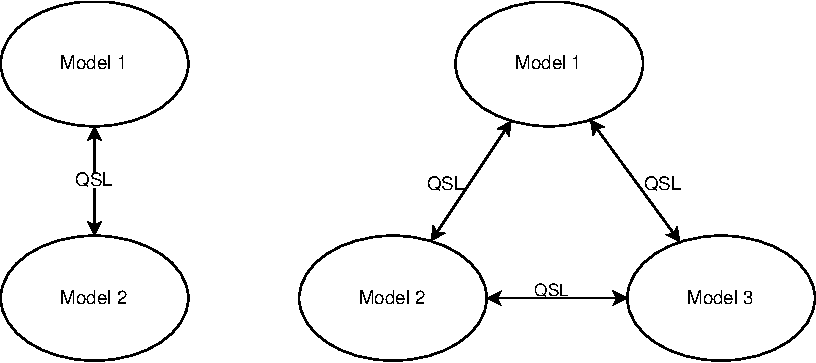
\includegraphics[height=4cm]{graphics/qsl}
  \caption{The increasing amount of different QSLs in larger model sets}
  \label{figure}
\end{figure}

Combining these individual levels therefore needs to follow an aggregation rule. For this reason, the possible options for calculating the QSL of a model set that have been designed are \texttt{min}, \texttt{max}, and \texttt{avg}. While with \texttt{min} the lowest level is chosen as the overall QSL for a model set, \texttt{max} chooses the highest level. \texttt{Avg} produces the mean value of all three measured levels.

A necessary addition to the QSLs was some form of normalization. As the value of the QSL of a model set will be combined with the Aggregated Model Score, both values have to be in the same interval in order to produce a meaningful Model Set Score that can be easily interpreted. It was therefore decided to introduce a QSL Score which is derived directly from the actual QSL. The level is put into the following formula which was derived and modified from Sünkel et. al. \cite{sunkel2022}:
$\frac{(QSL \cdot 10) + 60}{100}$.
Essentially, the formula puts the QSL Score inside an interval between 0.6 (if the QSL is 0 - no query sharing is possible) and 1 (if the QSL is 4 – same window size and features). This interval was chosen to fit the overall values that are to be expected in the Aggregated Model Score. 

The following summary is intended to give a better understanding of all the metrics and scores invented and used for the model set retrieval process. \autoref{scoreconstruction} then shows how all those different scores are constructed and their relations to one another.

\begin{itemize}
	\item \textbf{Performance Score}: Score for a single model. Chosen performance metric (e.g. accuracy, RMSE,…) is normalized over all models retrieved from the model database in a query. Assumes a value between 0 and 1.
\item \textbf{Resource Awareness Score}: Score for a single model. The chosen resource awareness metric is normalized over all models retrieved from the model database. In the implemented version, this is a count of the used features of a model, with an additional penalty for small window sizes. Assumes a value between 0 and 1.
\item \textbf{Model Score}: Overall score for single model. Combines Performance Score and Resource Awareness Score using a predefined weight. 
\item \textbf{Aggregated Model Score}: Score for model set. Determined by calculating the mean value of the Model Scores inside a set. 
\item \textbf{QSL}: Metric for model set. Depicts the degree of shared elements between two models inside a model set. Is determined for every 2-model combination inside a model set and subsequently ascertained for the entire model set by using one of three aggregation functions. Assumes value 0, 3, or 4 for each model-to-model relationship in a model set.
\item \textbf{QSL Score}: Score for model set. Derived from the QSL by using the normalization formula $\frac{(QSL \cdot 10) + 60}{100}$.
\item \textbf{Model Set Score}: Overall score for model set. Combines Aggregated Model Score and QSL Score using a predefined weight.
\end{itemize}


\begin{figure}[htbp]
  \centering
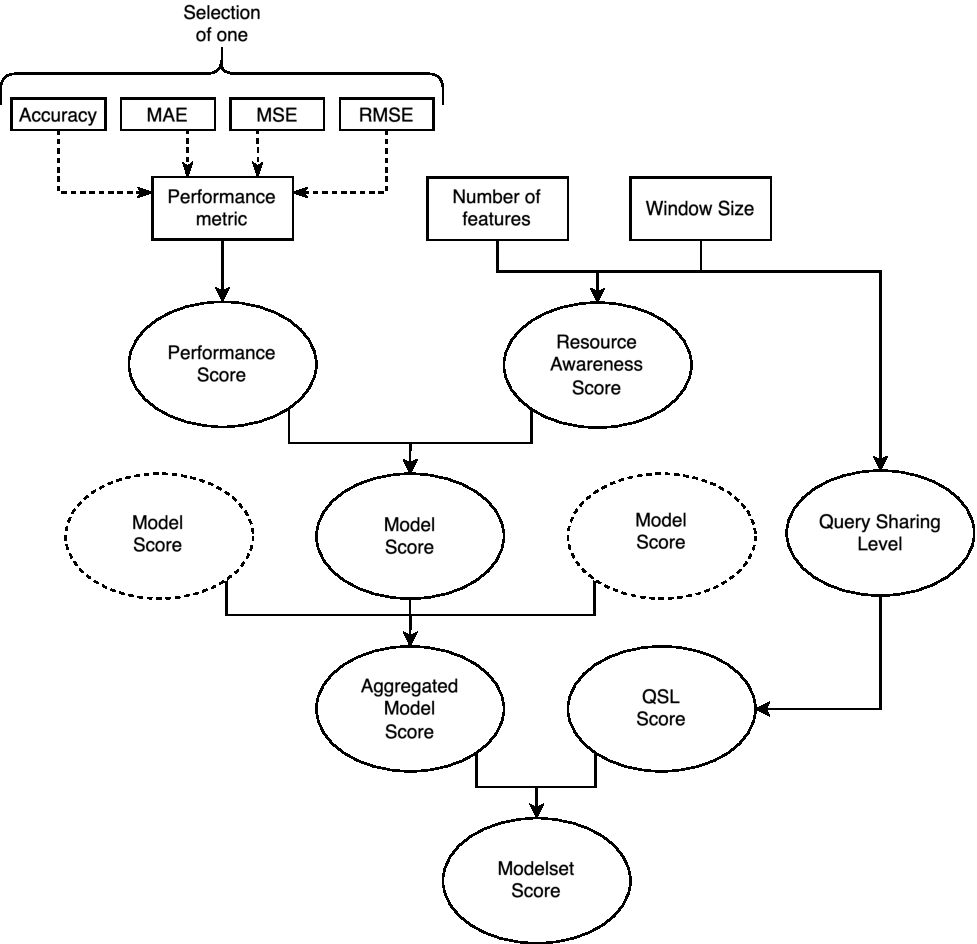
\includegraphics[height=12cm]{graphics/scores.pdf}
  \caption{Structure of the different scores used for the retrieval process}
  \label{scoreconstruction}
\end{figure}


As the model set retrieval system focuses on the logic of retrieving the k best model sets customized to the users’ preferences manifested in numerous settings that have been made prior to the request, the design and implementation of a front end e.g. in the sense of a web app has been dispensed with. Whilst an easy-to-understand user interface that guides the user through the various functions of the model set retrieval system might lead to a more intuitive and time-saving engagement between the user and the system, this part was not the focus of this work and might be better suited for future development.
